\subsection{Face Recognition dengan kamera}
\begin{enumerate}
    \item Proses pengumpulan dataset
    
    - Memasukan library openCV \textbf{cv2} serta \textbf{os}. Librari \textbf{os}
    digunakan untuk mengakses fungsi pada sistem operasi
    \begin{figure}[h!]
        \centering
        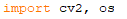
\includegraphics[width=0.3\linewidth]{images/fr_cam1.PNG}
        \caption{Memasukan library }
    \end{figure}

    - Proses face detection dengan memasukan algoritma \emph{haar-cascade classifier} serta
     memasukan video dengan \textbf{cv2.VideoCapture()}
     \begin{figure}[h!]
        \centering
        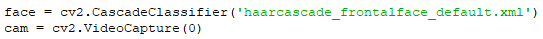
\includegraphics[width=0.9\linewidth]{images/fr_cam2.PNG}
        \caption{Proses face detection dengan masukan kamera}
    \end{figure}

    - Membuat inputan untuk id serta label folder pada kumpulan dataset, pembuatan folder label dataset menggunakan 
    library \textbf{os} yang menggunakan fungsi sitem operasi \textbf{mkdir}
    \begin{figure}[h!]
        \centering
        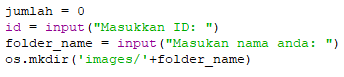
\includegraphics[width=0.7\linewidth]{images/fr_cam3.PNG}
        \caption{Masukan id serta nama untuk label dataset}
    \end{figure}

    - Proses deteksi wajah dan pengambilan dataset sebanyak 40 sample yang dimasukan pada direktori label
    \begin{figure}[h!]
        \centering
        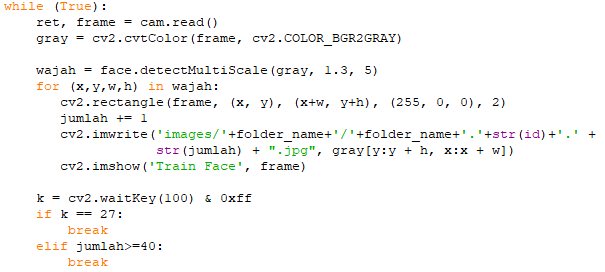
\includegraphics[width=0.9\linewidth]{images/fr_cam4.PNG}
        \caption{Proses face detection dan pengambilan dataset}
    \end{figure}

    - Hasil pengambilan dataset
    \begin{figure}[h!]
        \centering
        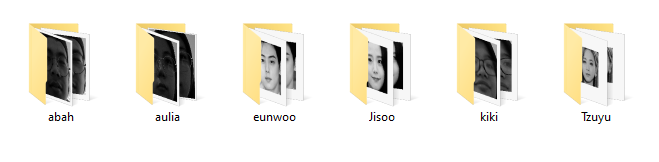
\includegraphics[width=1\linewidth]{images/fr_cam5.PNG}
        \caption{Kumpulan label direktori dataset}
        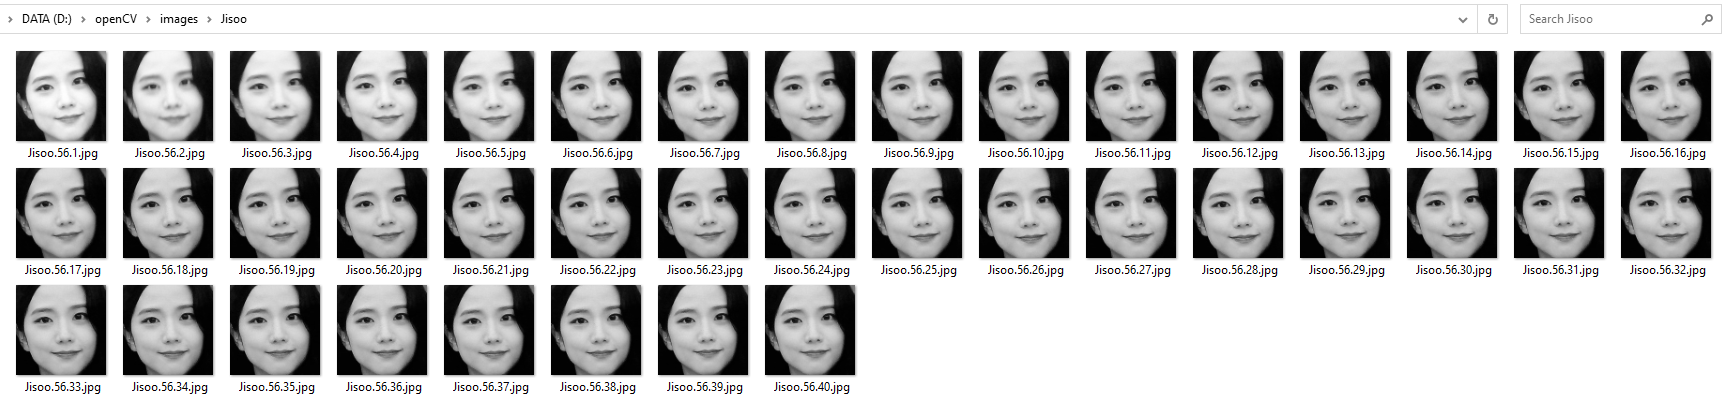
\includegraphics[width=1.1\linewidth]{images/fr_cam6.PNG}
        \caption{Isi direktori salah satu label dataset}
    \end{figure}
    \item Proses training dataset
    \item proses pengenalan wajah
\end{enumerate}